\documentclass{beamer}
%
% Choose how your presentation looks.
%
% For more themes, color themes and font themes, see:
% http://deic.uab.es/~iblanes/beamer_gallery/index_by_theme.html
%
\mode<presentation>
{
  \usetheme{default}      % or try Darmstadt, Madrid, Warsaw, ...
  \usecolortheme{default} % or try albatross, beaver, crane, ...
  \usefonttheme{default}  % or try serif, structurebold, ...
  \setbeamertemplate{footline}[frame number]
  \setbeamertemplate{navigation symbols}{}
  \setbeamertemplate{caption}[numbered]
} 

\usepackage[english]{babel}
\usepackage[utf8x]{inputenc}
\usepackage{graphicx}
\graphicspath{ {img/} }
\usepackage{xcolor}
\usepackage{colortbl}
\usepackage{verbatim}
\usepackage{tikz}

\title[Your Short Title]{EPIC
	\\
	{\large Electronic Programmable Intelligent Calculator}
}
\author{Michael Friesenhengst}
\institute{HTL Hollabrunn}
\date{14.06.2017}

\begin{document}

\begin{frame}
  \titlepage
\end{frame}

% Uncomment these lines for an automatically generated outline.
%\begin{frame}{Outline}
%  \tableofcontents
%\end{frame}

\section{Introduction}

\begin{frame}{Übersicht}


\begin{itemize}
  \item Notizen verfassen
  \item Skizzen erstellen
  \item Berechnungen durchführen
  \item Bedienung per Touchscreen
  \item Speichern von Dateien
  \item Kompatibilität mit externen Speichermedien
\end{itemize}



\end{frame}

\section{Umsetzung}

\begin{frame}{Umsetzung}



\begin{table}
	\centering
	\begin{tabular}{l|r}
		Mathematik (Theorie) & Weinzerl \\\hline
		\rowcolor{blue!25}
		Hardwareentwicklung & Friesenhengst \\\hline
		Software - Mathematik & Weinzerl \\\hline
		\rowcolor{blue!25}
		Software - GUI & Friesenhengst \\\hline
		\rowcolor{blue!25}
		Software - Raspberry Pi, Arduino & Friesenhengst \\\hline
		\rowcolor{blue!25}
		Marketing & Friesenhengst, Weinzerl
	\end{tabular}
\end{table}

\end{frame}

\section{Hardware}

\subsection{Recheneinheit}

\begin{frame}{Hardware - Recheneinheit}

\begin{columns}[T] % align columns
	\begin{column}{.48\textwidth}
		\begin{block}{Raspberry Pi 3}
			\begin{itemize}
				\item Treibersupport
				\item GPIO
				\item Wireless-LAN
				\item Dokumentation
				\item Betriebssystem auf SD-Karte
			\end{itemize}
		\end{block}
	\end{column}%
	\hfill%
	\begin{column}{.48\textwidth}
		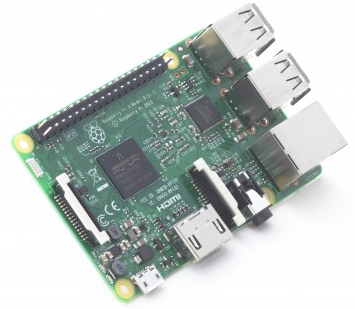
\includegraphics{rpi}
	\end{column}%
\end{columns}

\end{frame}

\subsection{Mikrocontroller}

\begin{frame}{Hardware - Mikrocontroller}

\begin{columns}[T] % align columns
	\begin{column}{.48\textwidth}
		\begin{block}{Arduino Pro Mini}
			\begin{itemize}
				\item Einfache Programmierung
				\item Geringer Energieaufwand
				\item Dokumentation
			\end{itemize}
		\end{block}
	\end{column}%
	\hfill%
	\begin{column}{.48\textwidth}
		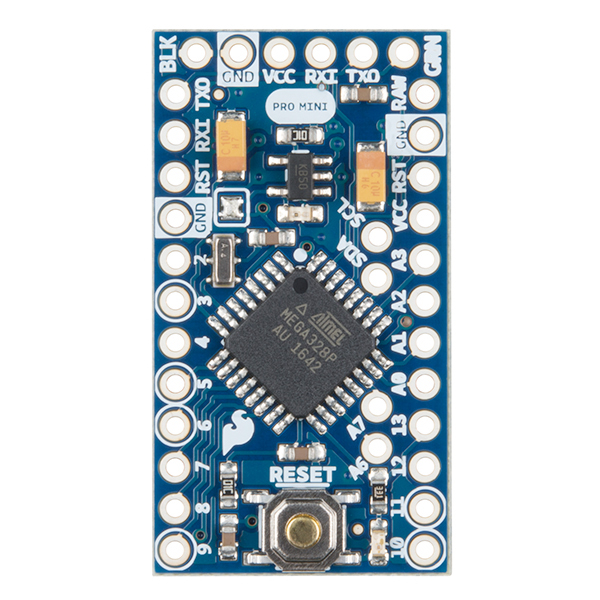
\includegraphics{arduino}
	\end{column}%
\end{columns}

\end{frame}
\begin{frame}{Hardware - Mikrocontroller}

\begin{columns}[T] % align columns
	\begin{column}{.48\textwidth}
		\begin{block}{Arduino Pro Mini}
			\begin{itemize}
				\item Einfache Programmierung
				\item Geringer Energieaufwand
				\item Dokumentation
			\end{itemize}
		\end{block}
	\end{column}%
	\hfill%
	\begin{column}{.48\textwidth}
		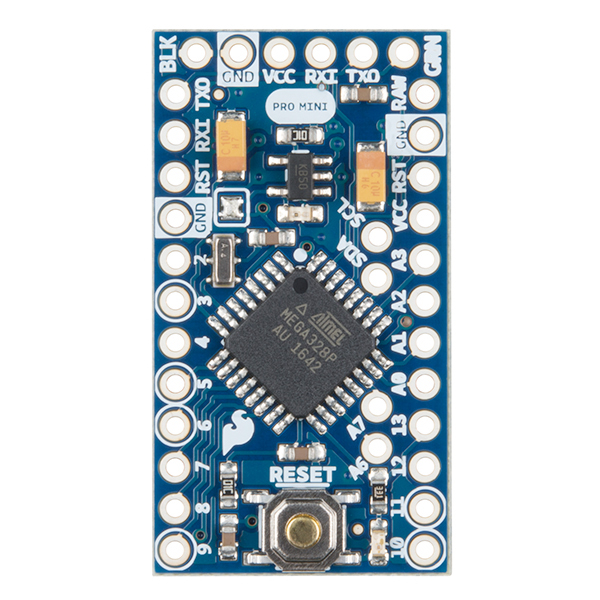
\includegraphics{arduino}
	\end{column}%
\end{columns}

\end{frame}

\section{Software}
\subsection{GUI}
\begin{frame}{GUI - Graphical User Interface}
\scalebox{0.8}{
	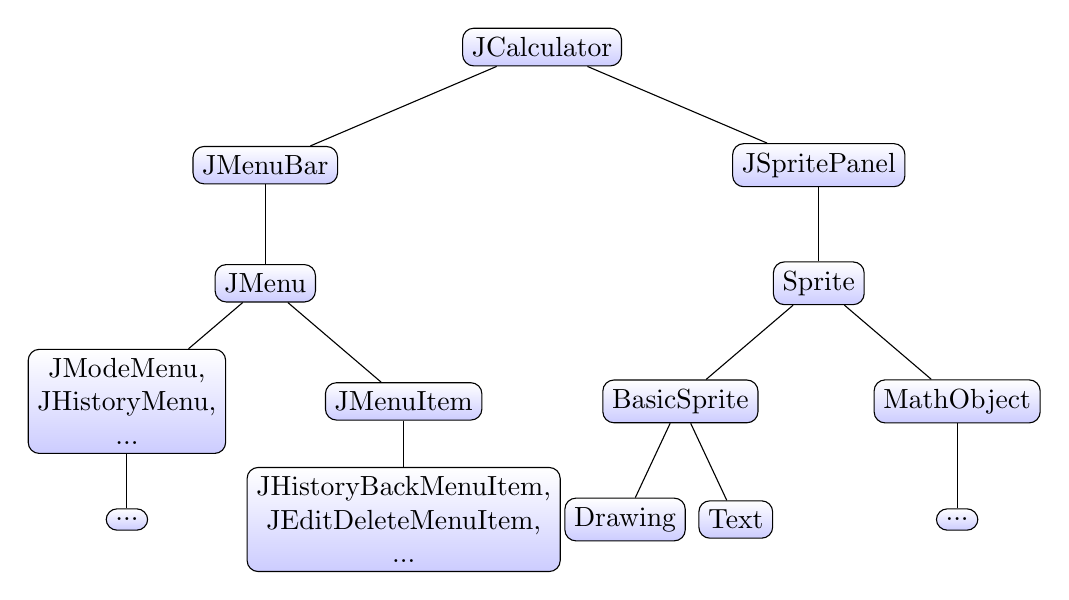
\begin{tikzpicture}[
	level 1/.style={sibling distance=20em},
	level 2/.style={sibling distance=0em},
	level 3/.style={sibling distance=10em},
	level 4/.style={sibling distance=4em},
	every node/.style = {shape=rectangle, rounded corners,
		draw, align=center,
		top color=white, bottom color=blue!20}]]
	\node {JCalculator}
	child { node {JMenuBar}
		child{ node {JMenu}
			child{ node {JModeMenu, \\ JHistoryMenu, \\...}
				child{ node {...}}
			}
			child{ node {JMenuItem}
				child{ node {JHistoryBackMenuItem, \\JEditDeleteMenuItem, \\ ...}}
			}
		}
	}
	child { node {JSpritePanel}
		child { node {Sprite}
			child { node {BasicSprite}
				child { node {Drawing}}
				child { node {Text}}
			}
			child { node {MathObject}
				child { node {...}}
			}
		 } };
	\end{tikzpicture}
}
\end{frame}


\subsection{softrpi}

\begin{frame}{Software - Raspberry Pi}
	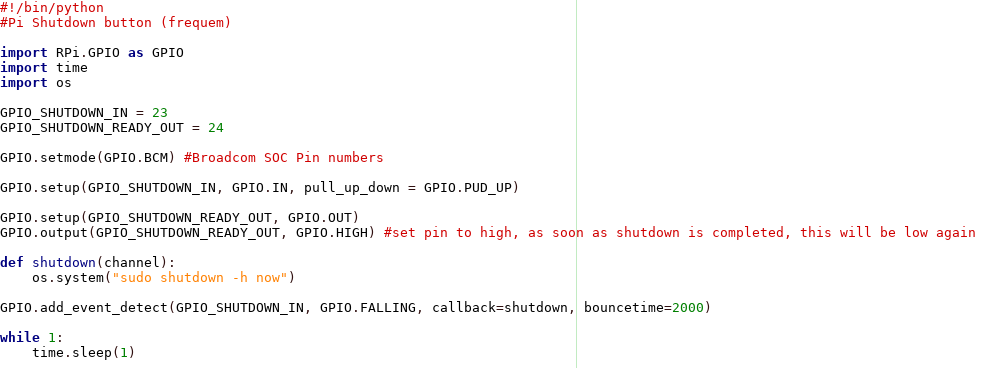
\includegraphics[width=160mm]{rpi_python_shutdown}
\end{frame}

\subsection{softarduino}

\begin{frame}{Software - Raspberry Pi}
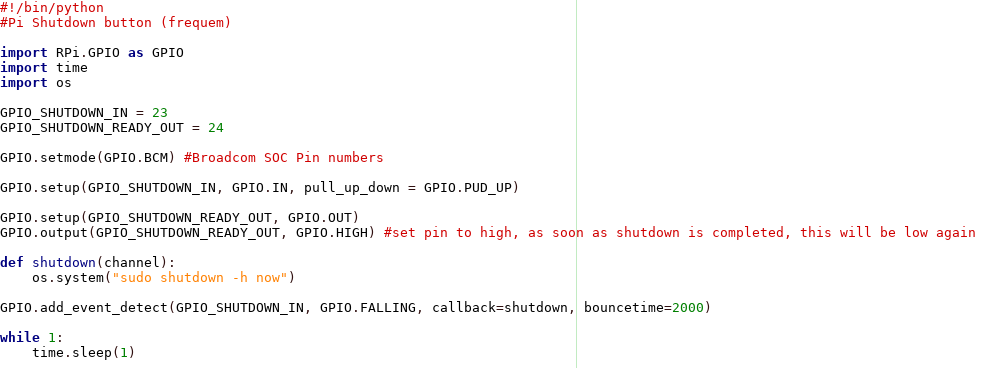
\includegraphics[width=160mm]{rpi_python_shutdown}
\end{frame}

\subsection{softarduino}

\begin{frame}{Software - Arduino}
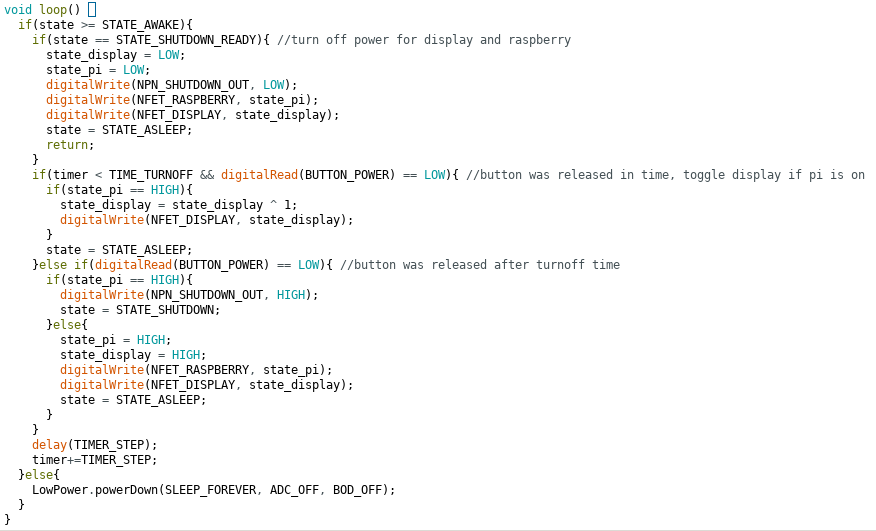
\includegraphics[width=145mm]{arduino_loop}
\end{frame}

\section{Marketing}

\begin{frame}{Marketing - Relevanter Markt}
	\begin{itemize}
		\item Wie viele Nachfrager beinhaltet der Markt?
		\item Zeitlich: Wie viele Anbieter beinhaltet der Markt, und welche Anbieter gehören zu den Hauptkonkurrenten?
		\item Hat ein Unternehmen eine marktbeherrschende Stellung, sodass wettbewerbsrechtliche Vorgaben nicht mehr eingehalten werden?
	\end{itemize}
\end{frame}

\section{Demo}
\begin{frame}{Demo}
\end{frame}


\end{document}
